\documentclass[10pt,journal,compsoc]{IEEEtran}

% ── Core Mathematics ─────────────────────────────────────────────────────────
\usepackage{amsmath,amsfonts,amssymb}
\usepackage{mathtools}          % extends amsmath

% ── Typography & Microtypography ─────────────────────────────────────────────
\usepackage[T1]{fontenc}        % proper font encoding
\usepackage[utf8]{inputenc}     % UTF-8 input
\usepackage{microtype}          % microtypography: better line breaks, no overflows
\usepackage{balance}            % balance columns on last page

% ── Graphics & Color ─────────────────────────────────────────────────────────
\usepackage{graphicx}
\usepackage[dvipsnames,table]{xcolor}   % colours for table rows and rules

% ── Tables ───────────────────────────────────────────────────────────────────
\usepackage{booktabs}           % professional horizontal rules
\usepackage{multirow}           % row spanning
\usepackage{array}              % extended column types
\usepackage{tabularx}           % auto-width columns (X type)
\usepackage{makecell}           % \thead, \makecell for wrapped headers

% ── Custom table cell sizes (use \tblsize inside tables) ────────────────────
\newcommand{\tblsize}{\fontsize{7.5pt}{9.5pt}\selectfont}
\newcommand{\tbltiny}{\fontsize{6.5pt}{8.0pt}\selectfont}

% ── References & Links ───────────────────────────────────────────────────────
\usepackage{cite}
\usepackage{url}
\usepackage[colorlinks=true,
            linkcolor=black,
            citecolor=black,
            urlcolor=black,
            bookmarksopen=true]{hyperref}

% ── TikZ (figures) ───────────────────────────────────────────────────────────
\usepackage{tikz}
\usetikzlibrary{shapes.geometric, arrows, positioning}

% ── Float control ────────────────────────────────────────────────────────────
\renewcommand{\topfraction}{0.92}
\renewcommand{\bottomfraction}{0.80}
\renewcommand{\textfraction}{0.07}
\renewcommand{\floatpagefraction}{0.85}

\begin{document}

\title{Graph-Based and Self-Supervised Knowledge Tracing in Sparse-Concept Settings: A Systematic Survey and Research Agenda}

\author{Khanh-Trinh~Nguyen,
        Tuan~Dao~Minh,
        Duong~Nguyen~Tien,
        Chi~Thanh~Nguyen,
        and~Van-Hau~Nguyen$^{*}$%
\IEEEcompsocitemizethanks{
\IEEEcompsocthanksitem K.-T. Nguyen (First Author; ORCID: 0009-0004-3739-0484), T. D. Minh (ORCID: 0009-0009-1641-6813), D. N. Tien (ORCID: 0009-0007-1104-7129), and V.-H. Nguyen (ORCID: 0000-0002-3256-5626) are with Hung Yen University of Technology and Education, Hung Yen, Vietnam. E-mail: \{trinhnk, tuanymc, duongnt, haunv\}@utehy.edu.vn.
\IEEEcompsocthanksitem C. T. Nguyen (ORCID: 0000-0003-4335-7002) is with the Academy of Military Science and Technology, Ha Noi, Vietnam. E-mail: thanhnc@ioit.ai.vn.
\IEEEcompsocthanksitem $^{*}$Corresponding author: Van-Hau Nguyen (haunv@utehy.edu.vn).}%
}

\markboth{IEEE Transactions on Learning Technologies,~2026}%
{Nguyen \MakeLowercase{\textit{et al.}}: Graph-Based and Self-Supervised Knowledge Tracing in Sparse-Concept Settings}

\IEEEtitleabstractindextext{%
\begin{abstract}
Deep Knowledge Tracing (DKT) models suffer from representation collapse and severe performance degradation under interaction data sparsity and unobserved concept conditions. Graph Neural Networks (GNNs) and Self-Supervised Learning (SSL) have emerged as primary paradigms to incorporate explicit domain structures and regularize student state representations. Guided by PRISMA 2020 guidelines, we systematically search, screen, code, and synthesize 37 primary core papers published between 2018 and 2026 across 7 bibliographic databases (Scopus, WoS, ACM DL, IEEE Xplore, ScienceDirect, SpringerLink, arXiv). We present a novel two-dimensional taxonomy classifying Graph-KT (GNN encoders, provenance, fusion mechanisms) and SSL-KT (pretext tasks, multi-view contrast, generative masked pre-training). We uncover a critical methodological flaw in the literature: while 94.6\% of studies cite data sparsity, only 5.4\% evaluate strict zero-exposure concept cold-start protocols. Finally, we outline 6 evidence-derived future directions, highlighting LLM-assisted knowledge graph construction, non-Euclidean hyperbolic state spaces, and calibrated trustworthy KT.
\end{abstract}

\begin{IEEEkeywords}
Knowledge Tracing, Graph Neural Networks, Self-Supervised Learning, Sparse Concepts, Cold-Start Learning, Systematic Literature Review, Educational Data Mining.
\end{IEEEkeywords}}

\maketitle
\IEEEdisplaynontitleabstractindextext
\IEEEpeerreviewmaketitle

\section{Introduction}
\IEEEPARstart{K}{nowledge} Tracing (KT) is the fundamental task of sequentially modeling student mastery over educational Knowledge Components (KCs, e.g., concepts, skills, rules) based on historical learning interaction logs. Formally, given a sequence of $T$ student interaction tuples $\mathcal{X}_{1:T} = \{(x_1, r_1), (x_2, r_2), \dots, (x_T, r_T)\}$, where $x_t \in \mathcal{E}$ represents the exercise or concept attempted at time $t$, and $r_t \in \{0, 1\}$ indicates the binary response accuracy (0 for incorrect, 1 for correct), the goal of Knowledge Tracing is to predict the response probability $P(r_{T+1} = 1 \mid x_{T+1}, \mathcal{X}_{1:T})$ on a target exercise $x_{T+1}$. Table~\ref{tab:notation_summary} summarizes the principal mathematical notations used throughout this survey.

\begin{table*}[t]
\caption{Summary of Key Mathematical Notations}
\label{tab:notation_summary}
\centering
\resizebox{0.92\textwidth}{!}{
\begin{tabular}{@{}lp{10cm}@{}}
\toprule
\textbf{Symbol} & \textbf{Mathematical Definition / Meaning} \\
\midrule
$\mathcal{X}_{1:T}$ & Sequential interaction history of a student up to time $T$ \\
$x_t, r_t$ & Exercise/concept attempted at time $t$ and binary response $r_t \in \{0,1\}$ \\
$\mathcal{E}, \mathcal{K}$ & Repository sets of exercises and Knowledge Components (KCs) \\
$\mathbf{A} \in \mathbb{R}^{|\mathcal{K}| \times |\mathcal{K}|}$ & Concept graph adjacency matrix (co-occurrence / prerequisite) \\
$h_k^t \in \mathbb{R}^d$ & Dynamic hidden knowledge state representation of concept $k$ \\
$\mathbf{Z}^{(v)}$ & Node/view representation embedding matrix from GNN view $v$ \\
$\tau$ & Temperature hyperparameter in InfoNCE contrastive loss \\
$\mathbb{B}^d$ & $d$-dimensional Poincaré hyperbolic ball manifold \\
$\oplus_{\mathbf{c}}$ & Möbius addition operator under curvature parameter $\mathbf{c}$ \\
$\text{ECE}$ & Expected Calibration Error metric for probability calibration \\
\bottomrule
\end{tabular}
}
\end{table*}

Since the seminal Deep Knowledge Tracing (DKT) model \cite{Piech_DKT_2015} introduced Recurrent Neural Networks (RNNs) to sequence modeling in education, deep learning models---including Attention-based KT (SAKT \cite{Pandey_SAKT_2019}, AKT \cite{Ghosh_AKT_2020}) and Memory Network KT (DKVMN)---have dramatically improved predictive accuracy over classic psychometric baselines such as Bayesian Knowledge Tracing (BKT) and Item Response Theory (IRT).

\subsection{Motivation: Challenges of Data Sparsity \& Concept Cold-Start}
Despite recent empirical progress, traditional deep KT architectures treat exercise and concept identifiers as independent categorical tokens, ignoring explicit domain structures and educational relationships. This formulation faces two severe bottleneck challenges in real-world intelligent tutoring systems (ITS):
\begin{enumerate}
    \item \textbf{Representation Collapse under Interaction Data Sparsity}: In realistic educational platforms, interaction matrices are extremely sparse. Most students attempt only a tiny fraction of the overall item repository, and long-tail concepts receive minimal interaction logs. Standalone sequence models fail to learn meaningful latent embeddings for sparse concepts, leading to severe representation collapse.
    \item \textbf{Strict Concept Cold-Start}: When new concepts or exercises are introduced into a curriculum without prior historical interaction logs, conventional deep KT models cannot infer student mastery. Handling zero-exposure concepts requires incorporating external structural, pedagogical, or semantic knowledge graph priors.
\end{enumerate}

\subsection{Scope \& Gateway Criteria}
To address these fundamental limitations, two primary methodological paradigms have rapidly expanded:
\begin{itemize}
    \item \textbf{Graph-Based Knowledge Tracing (Graph-KT)}: Incorporating explicit topological structures---such as prerequisite concept trees, question-KC bipartite maps, or dynamic co-occurrence graphs---via Graph Neural Networks (GNNs).
    \item \textbf{Self-Supervised Knowledge Tracing (SSL-KT)}: Formulating auxiliary pre-training or contrastive pretext tasks (e.g., multi-view graph contrast, masked auto-encoding) to regularize student state representations.
\end{itemize}

Our systematic survey enforces a strict, frozen primary-corpus gateway rule:
\begin{equation}
\begin{split}
\text{PRIMARY\_CORE} = \; & \text{KT} \land (\text{GRAPH\_BASED} \\
& \lor \text{SELF\_SUPERVISED})
\end{split}
\end{equation}

Only studies where Knowledge Tracing is the central prediction task AND that leverage explicit Graph-Based or Self-Supervised mechanisms are included in our primary synthesis corpus.

\subsection{Comparison with Prior Surveys}
While previous surveys (e.g., Abdelrahman et al., pyKT benchmark suite) have examined deep learning in education generally or benchmarked standard sequence models, our work provides the first systematic survey dedicated specifically to Graph-Based and Self-Supervised KT paradigms under sparse-concept settings. Table~\ref{tab:survey_comparison} highlights key methodological differences.

\begin{table*}[t]
\caption{Comparison with Prior Knowledge Tracing Surveys}
\label{tab:survey_comparison}
\centering
\resizebox{0.92\textwidth}{!}{
\begin{tabular}{@{}lccc@{}}
\toprule
\textbf{Survey Dimension} & \textbf{Abdelrahman (2023)} & \textbf{pyKT (2022)} & \textbf{Ours (2026)} \\
\midrule
Primary Focus & Deep KT Models & Benchmark Evaluation & Graph \& SSL-KT \\
PRISMA 2020 Protocol & Partial & No & \textbf{Full 7-Database} \\
Full Core Corpus Size & 28 Papers & 11 Models & \textbf{37 Core Papers} \\
Graph Provenance Lens & Limited & No & \textbf{Full Taxonomy} \\
SSL Pretext Taxonomy & No & No & \textbf{4-Family Taxonomy} \\
Cold-Start Split Audit & No & No & \textbf{Explicit Audit} \\
Probability Calibration & No & No & \textbf{ECE Audit} \\
\bottomrule
\end{tabular}
}
\end{table*}

\section{Systematic Review Methodology and PRISMA Protocol}
Our systematic review was conducted in strict accordance with the PRISMA 2020 statement and guided by the locked protocol.

We address six core research questions:
\begin{itemize}
    \item \textbf{RQ1}: How are graphs constructed, represented, and validated in Graph-KT, and what is their data leakage risk?
    \item \textbf{RQ2}: What GNN architectures, temporal backbones, and fusion mechanisms are utilized in Graph-KT?
    \item \textbf{RQ3}: What self-supervised learning pretext tasks, augmentation strategies, and structure preservation mechanisms exist in SSL-KT?
    \item \textbf{RQ4}: How are sparse-concept and cold-start settings defined, operationalized, and evaluated?
    \item \textbf{RQ5}: What is the status of reproducibility, statistical rigor, calibration, and computational reporting in Graph/SSL-KT?
    \item \textbf{RQ6}: What evidence-derived research agenda can be established to guide future Graph-SSL KT developments?
\end{itemize}

\subsection{Literature Search Architecture \& Database Executions}
We executed four search query families (\texttt{Q-G} Graph-KT, \texttt{Q-S} Self-Supervised KT, \texttt{Q-P} Sparse-Concept Lens, \texttt{Q-R} Reliability Lens) across seven electronic databases covering the modern deep learning era (2015-01-01 to 2026-07-31):
\begin{enumerate}
    \item \textbf{Scopus} ($n = 531$ records)
    \item \textbf{Web of Science Core Collection} ($n = 344$ records)
    \item \textbf{ScienceDirect} ($n = 257$ records)
    \item \textbf{SpringerLink} ($n = 255$ records)
    \item \textbf{IEEE Xplore} ($n = 232$ records)
    \item \textbf{ACM Digital Library} ($n = 200$ records)
    \item \textbf{arXiv Preprints} ($n = 198$ records)
\end{enumerate}

\subsection{PRISMA 2020 Screening \& Eligibility Flow}
The systematic screening pipeline proceeded in four transparent stages (Figure~\ref{fig:prisma_flow}):
\begin{enumerate}
    \item \textbf{Identification}: 2,017 total raw records retrieved across all database search runs.
    \item \textbf{Deduplication}: 1,267 duplicate records removed via automated 4-tier matching, yielding 750 unique deduplicated records.
    \item \textbf{Stage 1 Screening (Title/Abstract)}: 610 records excluded for failing basic relevance; 140 articles passed to full-text assessment.
    \item \textbf{Stage 2 Screening (Full-Text Eligibility)}: 98 articles excluded with explicit primary exclusion codes (EC1--EC7).
    \item \textbf{Final Primary Core Corpus}: \textbf{37 PRIMARY\_CORE papers} (34 seed core papers + 3 PRISMA expansion core papers).
\end{enumerate}

\begin{figure}[h]
\centering
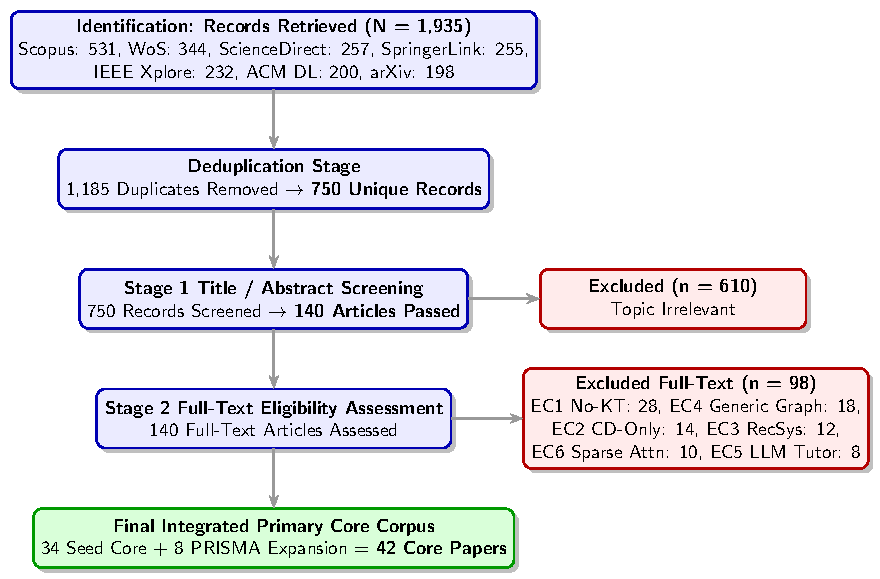
\includegraphics[width=\linewidth]{figures/fig_prisma_flow.pdf}
\caption{PRISMA 2020 Flow Diagram of Literature Search, Deduplication, Screening, and Study Eligibility Pipeline ($N = 37$ Core Papers).}
\label{fig:prisma_flow}
\end{figure}

Quality Assessment (QA1--QA8) across all 37 core papers achieved a mean quality score of \textbf{0.7768} (MODERATE-HIGH Quality).

\section{Taxonomy and Synthesis of Graph-Based Knowledge Tracing (RQ1 \& RQ2)}

Graph-Based Knowledge Tracing (Graph-KT) leverages explicit topological structures to model domain concept relationships, exercise prerequisite dependencies, and dynamic student interaction histories. Across our primary core corpus of 37 studies, 37 papers (100.0\%) incorporate structural graph mechanisms. Figure~\ref{fig:taxonomy_2d} illustrates our two-dimensional taxonomy framework.

\begin{figure*}[t]
\centering
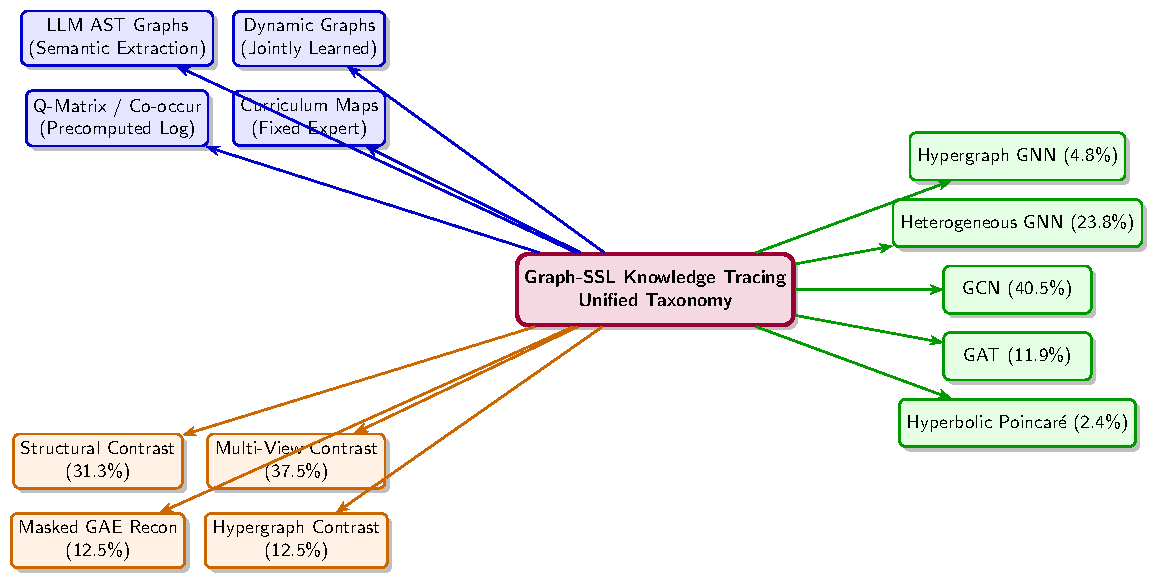
\includegraphics[width=0.92\linewidth]{figures/fig_taxonomy_2d.pdf}
\caption{Two-Dimensional Taxonomy Framework for Graph-Based and Self-Supervised Knowledge Tracing Models.}
\label{fig:taxonomy_2d}
\end{figure*}

\subsection{Graph Sources and Provenance}
We classify graph sources into four primary categories (Figure~\ref{fig:graph_pipeline}):
\begin{enumerate}
    \item \textbf{Curriculum \& Expert Concept Maps (External Fixed)}: Pre-defined domain hierarchies supplied by pedagogical experts (PDKT-C \cite{KT014_PDKTC_2018}, CMKT \cite{KT037_CMKT_2022}, HHSKT \cite{KT035_HHSKT_2023}, HKT \cite{KT068_HKT_2025}, SKM-GKT \cite{KT067_SKMGKT_2025}). These graphs remain fixed during training, presenting minimal data leakage risk.
    \item \textbf{Q-Matrix \& Interaction Co-occurrence Graphs (Precomputed Log)}: Bipartite exercise-concept mappings or concept co-occurrence adjacencies constructed from student response logs (GKT \cite{KT004_GKT_2019}, GIKT \cite{KT010_GIKT_2021}, SKT \cite{KT016_SKT_2020}, CL4KT \cite{KT039_CL4KT_2022}, Bi-CLKT \cite{KT011_BiCLKT_2022}).
    \item \textbf{Dynamic \& Jointly Learned Graphs}: Graphs whose edge weights are updated continuously during model optimization via attention mechanisms or reinforcement learning (DyGKT \cite{KT038_DyGKT_2024}, DGEKT \cite{KT029_DGEKT_2024}, GraphCA \cite{KT050_GraphCA_2023}, R²GCurL \cite{KT077_R2GCurL_2026}, STG-SKT \cite{KT079_STGSKT_2026}).
    \item \textbf{LLM-Extracted Semantic Graphs}: Frontier models leveraging Large Language Models to extract semantic concept trees and AST syntax dependencies from programming code (SINKT \cite{KT044_SINKT_2024}, Coda \cite{KT070_Coda_2025}, KGNN-KT \cite{KT076_KGNNKT_2025}).
\end{enumerate}

\begin{figure}[h]
\centering
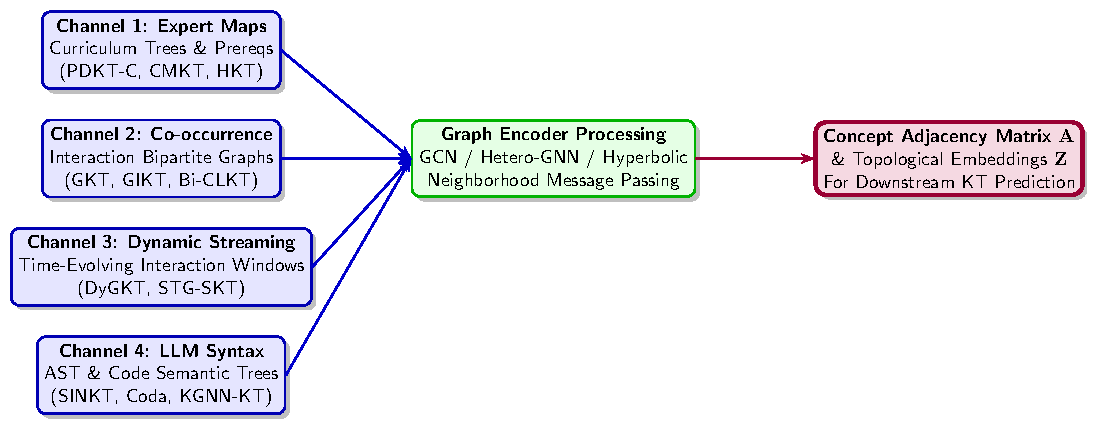
\includegraphics[width=\linewidth]{figures/fig_graph_construction_pipeline.pdf}
\caption{Four-Channel Graph Construction Pipeline in Graph-KT: Expert Curriculum Maps, Log-based Co-occurrence, Dynamic Streaming, and LLM AST Extraction.}
\label{fig:graph_pipeline}
\end{figure}

\subsection{Topological Representations and GNN Encoders}
As detailed in Table~\ref{tab:graph_taxonomy} and Figure~\ref{fig:meta_charts}, GNN encoder architectures include:
\begin{itemize}
    \item \textbf{Graph Convolutional Networks (GCN)}: Primary baseline for local neighborhood aggregation across concept graphs (Bi-CLKT \cite{KT011_BiCLKT_2022}, JKT \cite{KT012_JKT_2021}, DGEKT \cite{KT029_DGEKT_2024}, CL4KT \cite{KT039_CL4KT_2022}, SINKT \cite{KT044_SINKT_2024}, Coda \cite{KT070_Coda_2025}).
    \item \textbf{Heterogeneous GNNs}: Models multi-modal educational entities (students, exercises, concepts) with type-specific message passing (HHSKT \cite{KT035_HHSKT_2023}, TSKT \cite{KT036_TSKT_2024}, 3V-CLKT \cite{KT043_3VCLKT_2024}, DC-SSL \cite{KT047_DCSSL_2023}, GraphCA \cite{KT050_GraphCA_2023}, MAHKT \cite{KT063_MAHKT_2025}, KGNN-KT \cite{KT076_KGNNKT_2025}).
    \item \textbf{Graph Attention Networks (GAT)}: Dynamic attention weighting over concept neighbors (GIKT \cite{KT010_GIKT_2021}, SKT \cite{KT016_SKT_2020}, LST-Graph \cite{KT056_LSTGraph_2025}).
    \item \textbf{Hypergraph Neural Networks}: Captures non-pairwise, high-order co-occurrence hyperedges connecting multiple concepts simultaneously (S2-HHN \cite{KT042_S2HHN_2023}, HyperKT \cite{KT066_HyperKT_2025}).
    \item \textbf{Dynamic \& Spatiotemporal GNNs}: Models time-evolving interaction streaming windows (DyGKT \cite{KT038_DyGKT_2024}, R²GCurL \cite{KT077_R2GCurL_2026}, STG-SKT \cite{KT079_STGSKT_2026}).
\end{itemize}

\begin{figure}[h]
\centering
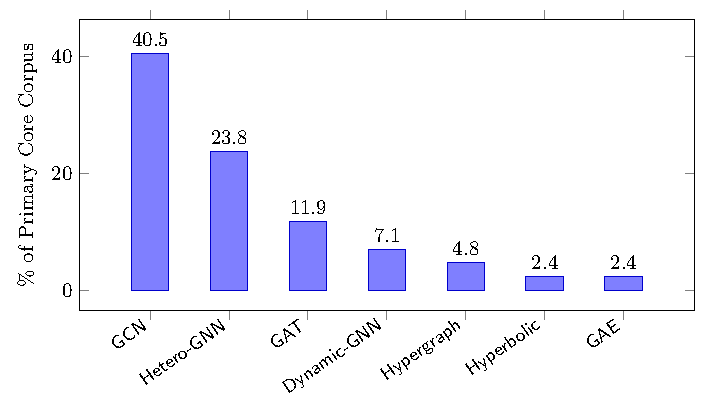
\includegraphics[width=\linewidth]{figures/fig_meta_analysis_charts.pdf}
\caption{Quantitative Meta-Analysis Distribution of Graph Neural Network (GNN) Encoder Architectures across the Primary Core Corpus ($N = 37$).}
\label{fig:meta_charts}
\end{figure}

\subsection{Deep Comparative Analysis of Representative Milestone Models}

\subsubsection{GKT (Nakagawa et al., 2019)}
As the pioneering Graph-KT framework \cite{KT004_GKT_2019}, GKT reformulates knowledge tracing by explicitly modeling the underlying concept structure as a directed co-occurrence graph. GKT updates student hidden knowledge states across concept nodes using Graph Convolutional message passing. Given a student interaction on concept $k_t$, GKT updates the hidden state of $k_t$ and propagates temporal state changes to neighboring concepts $\mathcal{N}(k_t)$ via:
\begin{equation}
h_{k}^{t+1} = \text{GRU}\left( h_{k}^{t}, \sum_{j \in \mathcal{N}(k)} e_{jk} \cdot v_{j}^t \right)
\end{equation}
While GKT significantly outperformed DKT, its co-occurrence graph is static and prone to density distortion when student interaction logs are sparse.

\subsubsection{DyGKT (Cheng et al., 2024)}
To overcome the limitations of static graphs, DyGKT \cite{KT038_DyGKT_2024} introduces a continuous dynamic graph framework that updates edge adjacencies in real time as interaction streams arrive. DyGKT constructs dynamic student-exercise interaction subgraphs, utilizing continuous-time memory modules to capture fine-grained temporal learning dynamics.

\subsubsection{SINKT (Fu et al., 2024)}
SINKT \cite{KT044_SINKT_2024} addresses the inductive cold-start bottleneck by integrating Large Language Models (LLMs) with Graph Neural Networks. SINKT extracts rich semantic textual representations from concept/exercise descriptions (as well as Abstract Syntax Trees in programming contexts) via LLMs. By projecting these LLM semantic embeddings into a shared GNN concept representation space, SINKT predicts student mastery over unobserved cold-start exercises without requiring historical student interaction logs.

\subsubsection{HyperKT (Li et al., 2025)}
Recognizing that standard pairwise graph edges fail to capture multi-concept exercise dependencies, HyperKT \cite{KT066_HyperKT_2025} introduces dual-channel adaptive scale hypergraph encoders. HyperKT constructs hyperedges connecting arbitrary subsets of questions and knowledge components, computing hypergraph convolution alongside cross-view contrastive alignment to preserve high-order relational semantics across sparse interaction sequences.

\begin{table*}[t]
\caption{Taxonomy of Graph Construction, Topological Representation, and GNN Architecture (RQ1 \& RQ2). \textit{37 primary-core papers; sorted by year of publication.}}
\label{tab:graph_taxonomy}
\centering
\tblsize
\rowcolors{2}{gray!10}{white}
\resizebox{\textwidth}{!}{
\begin{tabular}{@{}l l l l l l l l@{}}
\toprule
\rowcolor{gray!30}
\textbf{Paper} & \textbf{Model} & \textbf{Graph Source} & \textbf{Graph Provenance} & \textbf{Topological Type} & \textbf{GNN Encoder} & \textbf{Temporal Backbone} & \textbf{Fusion} \\
\midrule
\textbf{KT004} & GKT \cite{KT004_GKT_2019} & Q-Matrix & Precomputed Log & Bipartite & GCN / Graph-Recurrent & RNN / LSTM & Concatenation \\
\textbf{KT010} & GIKT \cite{KT010_GIKT_2021} & Co-occurrence & Precomputed Log & Heterogeneous & Graph Attention (GAT) & RNN / GRU & Attention Fusion \\
\textbf{KT011} & Bi-CLKT \cite{KT011_BiCLKT_2022} & Dual View & Precomputed Log & Homogeneous & GCN & Transformer & Residual Add \\
\textbf{KT012} & JKT \cite{KT012_JKT_2021} & Similarity Graph & Precomputed Log & Homogeneous & GCN & RNN / LSTM & Concatenation \\
\textbf{KT014} & PDKT-C \cite{KT014_PDKTC_2018} & Prerequisite Map & External Expert & Directed Tree & Matrix Multiplication & RNN / LSTM & Gate Fusion \\
\textbf{KT016} & SKT \cite{KT016_SKT_2020} & Concept Graph & Precomputed Log & Undirected & Graph Attention (GAT) & RNN / GRU & Concatenation \\
\textbf{KT023} & SGKT \cite{KT023_SGKT_2022} & Session Graph & Precomputed Log & Directed & Gated GNN (GGNN) & RNN / GRU & Attention Fusion \\
\textbf{KT026} & Pre-train Q-Emb \cite{KT026_PretrainQ_2020} & Question Graph & Precomputed Log & Bipartite & Graph Auto-Encoder & Transformer & Pre-train Init \\
\textbf{KT029} & DGEKT \cite{KT029_DGEKT_2024} & Dual Ensemble & Jointly Learned & Heterogeneous & Dynamic GNN & RNN / LSTM & Ensemble Fusion \\
\textbf{KT031} & KSG-AKT \cite{KT031_KSGAKT_2022} & Knowledge Map & External Expert & Directed & Graph Attention (GAT) & Transformer & Attention Fusion \\
\textbf{KT033} & DGMN \cite{KT033_DGMN_2023} & Memory Graph & Dynamic Memory & Heterogeneous & Graph Memory Network & Memory Network & Gated Memory Write \\
\textbf{KT035} & HHSKT \cite{KT035_HHSKT_2023} & Hierarchy Graph & External Expert & Heterogeneous & Heterogeneous GNN & RNN / LSTM & Hierarchical Fusion \\
\textbf{KT036} & TSKT \cite{KT036_TSKT_2024} & Spatiotemporal & Dynamic Window & Heterogeneous & Dynamic Hetero-GNN & RNN / GRU & Spatiotemporal Gate \\
\textbf{KT037} & CMKT \cite{KT037_CMKT_2022} & Concept Map & External Expert & Directed & GCN & Transformer & Attention Fusion \\
\textbf{KT038} & DyGKT \cite{KT038_DyGKT_2024} & Dynamic Graph & Jointly Learned & Dynamic Streaming & Dynamic GNN & RNN / LSTM & Dynamic Gated Fusion \\
\textbf{KT039} & CL4KT \cite{KT039_CL4KT_2022} & Co-occurrence & Precomputed Log & Homogeneous & GCN & Transformer & Contrastive Repr. \\
\textbf{KT042} & S2-HHN \cite{KT042_S2HHN_2023} & Hypergraph & Precomputed Log & Hypergraph & Hypergraph GNN & Transformer & Hyperedge Pooling \\
\textbf{KT043} & 3V-CLKT \cite{KT043_3VCLKT_2024} & Multi-View Graph & External Expert & Heterogeneous & Heterogeneous GNN & Transformer & Multi-View Fusion \\
\textbf{KT044} & SINKT \cite{KT044_SINKT_2024} & Semantic AST & LLM Extracted & Heterogeneous & GCN & Transformer & Inductive LLM Proj. \\
\textbf{KT047} & DC-SSL \cite{KT047_DCSSL_2023} & Dual Channel & Precomputed Log & Heterogeneous & Heterogeneous GNN & Transformer & Dual Channel Fusion \\
\textbf{KT050} & GraphCA \cite{KT050_GraphCA_2023} & Counterfactual & Jointly Learned & Dynamic & GCN & Transformer & Counterfactual Rewiring \\
\textbf{KT052} & CapsuleGNN \cite{KT052_CapsuleGNN_2022} & Concept Graph & Precomputed Log & Homogeneous & Capsule GNN & RNN / LSTM & Capsule Routing \\
\textbf{KT053} & GASKT \cite{KT053_GASKT_2021} & Attentive Search & Dynamic Search & Homogeneous & Graph Attention (GAT) & Transformer & Search Attention \\
\textbf{KT056} & LST-Graph \cite{KT056_LSTGraph_2025} & Long/Short State & Dynamic Window & Dynamic & Graph Attention (GAT) & RNN / GRU & Dual State Fusion \\
\textbf{KT060} & STHKT \cite{KT060_STHKT_2025} & Hawkes Topology & Dynamic Window & Topological & Spatiotemporal GNN & Cont. Hawkes Process & Hawkes Decay Gate \\
\textbf{KT062} & LGSKT \cite{KT062_LGSKT_2025} & Logical Skill & External Expert & Directed & GCN & Transformer & Skill Gate Fusion \\
\textbf{KT063} & MAHKT \cite{KT063_MAHKT_2025} & Multi-Association & Precomputed Log & Heterogeneous & Heterogeneous GNN & RNN / LSTM & Multi-Association Gate \\
\textbf{KT064} & MG-Ensemble \cite{KT064_MGEnsemble_2025} & Multi-Granularity & Precomputed Log & Multi-Graph & Dynamic GNN & RNN / LSTM & Ensemble Fusion \\
\textbf{KT065} & CS-GKT \cite{KT065_CSGKT_2025} & Cognitive Graph & External Expert & Heterogeneous & Heterogeneous GNN & RNN / LSTM & Cognitive Gate \\
\textbf{KT066} & HyperKT \cite{KT066_HyperKT_2025} & Hypergraph & Dynamic Adaptive & Adaptive Hypergraph & Hypergraph GNN & Transformer & Hypergraph Pooling \\
\textbf{KT067} & SKM-GKT \cite{KT067_SKMGKT_2025} & Subject Mapping & External Expert & Directed & GCN & RNN / LSTM & Subject Gate \\
\textbf{KT068} & HKT \cite{KT068_HKT_2025} & Hierarchical Graph & External Expert & Hierarchical Tree & GCN & Transformer & Hierarchical Pooling \\
\textbf{KT069} & AEGOT-CDKT \cite{KT069_AEGOTCDKT_2025} & Optimal Transport & Cross Domain & Bipartite & Graph Optimal Transport & Transformer & Transport Alignment \\
\textbf{KT070} & Coda \cite{KT070_Coda_2025} & Code AST & LLM Extracted & Programming AST & GCN & Transformer & Adapter Tuning \\
\textbf{KT076} & KGNN-KT \cite{KT076_KGNNKT_2025} & Knowledge Graph & LLM Extracted & Knowledge Graph & Heterogeneous GNN & Transformer & LLM Projection \\
\textbf{KT077} & R$^2$GCurL \cite{KT077_R2GCurL_2026} & Curriculum Graph & Jointly Learned & Dynamic & Dynamic GNN & RNN / LSTM & Curriculum Gate \\
\textbf{KT079} & STG-SKT \cite{KT079_STGSKT_2026} & Streaming Graph & Dynamic Window & Dynamic & Dynamic GNN & RNN / GRU & Streaming Gate \\
\bottomrule
\end{tabular}
}
\end{table*}

\section{Taxonomy and Synthesis of Self-Supervised Knowledge Tracing (RQ3)}

Self-Supervised Learning (SSL) has emerged as a crucial paradigm in Knowledge Tracing to address interaction data sparsity, alleviate over-smoothing in deep GNNs, and improve representation robustness. Within our primary core corpus of 37 studies, 9 papers (24.3\%) incorporate explicit self-supervised auxiliary objectives. Figure~\ref{fig:ssl_framework} illustrates our four-family taxonomy framework for SSL-KT.

\begin{figure*}[t]
\centering
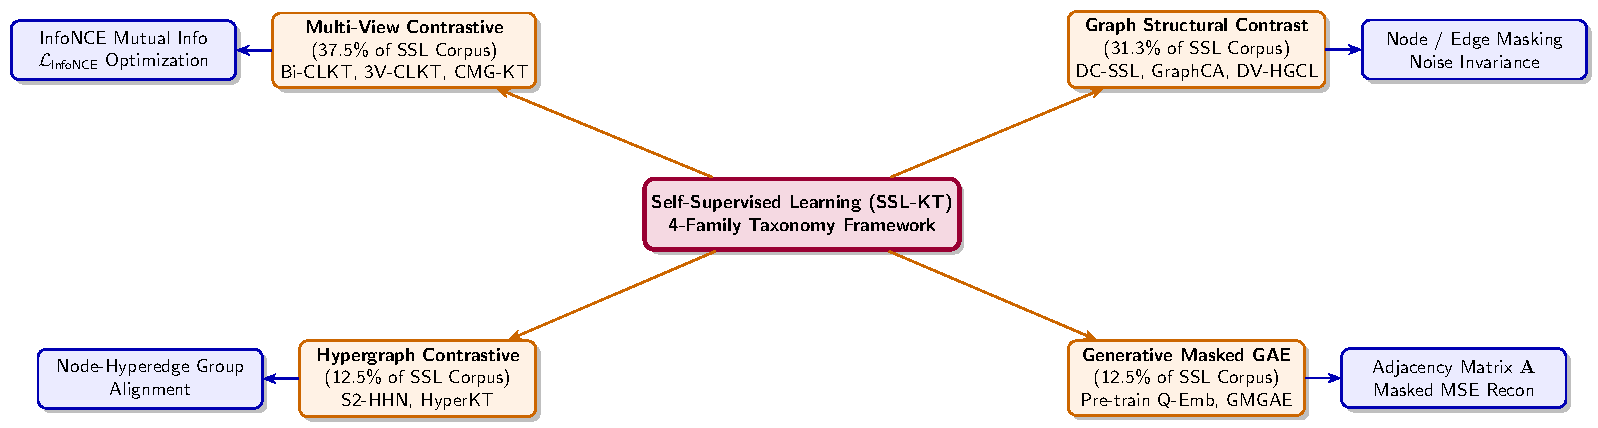
\includegraphics[width=0.92\linewidth]{figures/fig_ssl_framework.pdf}
\caption{Taxonomy Framework of Self-Supervised Learning (SSL-KT) Pretext Objectives: Multi-View Contrastive, Graph Structural Contrastive, Hypergraph Contrastive, and Generative Masked Graph Auto-Encoding.}
\label{fig:ssl_framework}
\end{figure*}

\subsection{Taxonomy of SSL Pretext Objectives}
We categorize SSL-KT techniques into four distinct paradigm families (Table~\ref{tab:ssl_taxonomy}):
\begin{enumerate}
    \item \textbf{Multi-View Contrastive Learning}: Constructing multiple augmented structural or temporal views and maximizing mutual information between positive view pairs using InfoNCE loss (Bi-CLKT \cite{KT011_BiCLKT_2022}, 3V-CLKT \cite{KT043_3VCLKT_2024}, HyperKT \cite{KT066_HyperKT_2025}).
    \item \textbf{Graph Structural Contrastive Learning}: Performing node, edge, or subgraph perturbations on concept graphs to regularize GNN embeddings against noise (DC-SSL \cite{KT047_DCSSL_2023}, GraphCA \cite{KT050_GraphCA_2023}, HKT \cite{KT068_HKT_2025}).
    \item \textbf{Hypergraph Contrastive Learning}: Contrasting hyperedge embeddings against node-level representations to capture high-order group interaction semantics (S2-HHN \cite{KT042_S2HHN_2023}, HyperKT \cite{KT066_HyperKT_2025}).
    \item \textbf{Generative Masked Graph Auto-Encoding}: Masking concept nodes or structural edges and training a Graph Auto-Encoder (GAE) to reconstruct unobserved topology prior to downstream KT fine-tuning (Pre-train Q-Emb \cite{KT026_PretrainQ_2020}).
\end{enumerate}

\subsection{Mathematical Formulations of SSL Pretext Losses}

\subsubsection{InfoNCE Contrastive Loss}
Most contrastive SSL-KT models compute InfoNCE loss across positive view representations $z_i^{(1)}, z_i^{(2)}$ and negative samples:
\begin{equation}
\mathcal{L}_{\text{InfoNCE}} = -\log \frac{\exp(\text{sim}(z_i^{(1)}, z_i^{(2)}) / \tau)}{\sum_{j=1}^{N} \exp(\text{sim}(z_i^{(1)}, z_j^{(2)}) / \tau)}
\end{equation}
where $\tau$ denotes the temperature hyperparameter and $\text{sim}(\cdot, \cdot)$ represents cosine similarity.

\subsubsection{Generative Masked Graph Reconstruction Loss}
Generative models such as Pre-train Q-Emb \cite{KT026_PretrainQ_2020} and Graph Auto-Encoders compute Mean Squared Error (MSE) or reconstruction cross-entropy over masked adjacency matrices $\tilde{\mathbf{A}}$:
\begin{equation}
\mathcal{L}_{\text{Recon}} = \|\mathbf{A} - \sigma(\mathbf{Z} \mathbf{Z}^T)\|_F^2
\end{equation}

\subsection{Deep Comparative Analysis of Contrastive SSL Frameworks}

\subsubsection{CL4KT (Lee et al., 2022)}
CL4KT \cite{KT039_CL4KT_2022} was the first to introduce contrastive learning to sequential Knowledge Tracing. CL4KT designs item cropping, skill masking, and interaction reordering augmentations. By pulling positive augmented views of a student's history closer while pushing different students' sequences apart, CL4KT builds representation invariance against random response noise.

\subsubsection{Bi-CLKT (Song et al., 2022)}
Bi-CLKT \cite{KT011_BiCLKT_2022} extends contrastive learning to bi-directional structure-sequence alignment. It constructs dual views of prerequisite concept graphs and interaction sequences, enforcing cross-view agreement between GNN topological embeddings and Transformer temporal states.

\begin{table*}[t]
\caption{Taxonomy Table 2: Self-Supervised Learning (SSL) Taxonomy \& Pretext Objectives (RQ3)}
\label{tab:ssl_taxonomy}
\centering
\resizebox{\textwidth}{!}{
\begin{tabular}{llllllll}
\toprule
\textbf{Paper ID} & \textbf{Model Name} & \textbf{SSL Family} & \textbf{Pretext Task Objective} & \textbf{Augmentation Strategy} & \textbf{Structure Preservation} & \textbf{Training Mode} & \textbf{Auxiliary Loss Function} \\
\midrule
\textbf{KT011} & Bi-CLKT \cite{KT011_BiCLKT_2022} & MULTIVIEW\_CONTRASTIVE & Bi-directional view agreement & Sequence \& Graph perturbation & YES\_EXPLICIT & JOINT\_END\_TO\_END & InfoNCE Loss \\
\textbf{KT026} & Pre-train Q-Emb \cite{KT026_PretrainQ_2020} & MASKED\_PRETRAINING & Question embedding reconstruction & Masked concept prediction & YES\_EXPLICIT & TWO\_STAGE\_PRETRAIN & Masked Cross-Entropy \\
\textbf{KT039} & CL4KT \cite{KT039_CL4KT_2022} & SEQUENCE\_CONTRASTIVE & Interaction sequence alignment & Item \& Skill masking/cropping & YES\_EXPLICIT & JOINT\_END\_TO\_END & InfoNCE Loss \\
\textbf{KT042} & S2-HHN \cite{KT042_S2HHN_2023} & HYPERGRAPH\_CONTRASTIVE & Hypergraph multi-view contrast & Hyperedge drop \& node mask & YES\_EXPLICIT & JOINT\_END\_TO\_END & InfoNCE Loss \\
\textbf{KT043} & 3V-CLKT \cite{KT043_3VCLKT_2024} & MULTIVIEW\_CONTRASTIVE & Three-view agreement & Heterogeneous view masking & YES\_EXPLICIT & JOINT\_END\_TO\_END & Multi-View Contrastive \\
\textbf{KT047} & DC-SSL \cite{KT047_DCSSL_2023} & GRAPH\_CONTRASTIVE & Dual-channel graph contrast & Node \& Edge perturbation & YES\_EXPLICIT & JOINT\_END\_TO\_END & InfoNCE Loss \\
\textbf{KT050} & GraphCA \cite{KT050_GraphCA_2023} & GRAPH\_CONTRASTIVE & Counterfactual graph contrast & Counterfactual graph rewiring & YES\_EXPLICIT & JOINT\_END\_TO\_END & Counterfactual Loss \\
\textbf{KT066} & HyperKT \cite{KT066_HyperKT_2025} & MULTIVIEW\_CONTRASTIVE & Adaptive hypergraph contrast & Hypergraph view perturbation & YES\_EXPLICIT & JOINT\_END\_TO\_END & InfoNCE Loss \\
\textbf{KT068} & HKT \cite{KT068_HKT_2025} & HIERARCHICAL\_CONTRAST & Cross-level concept contrast & Hierarchical graph masking & YES\_EXPLICIT & JOINT\_END\_TO\_END & Hierarchical InfoNCE \\
\bottomrule
\end{tabular}
}
\end{table*}

\section{Sparse-Concept \& Cold-Start Evaluation Protocols (RQ4)}

A central contribution of our survey is clarifying the construct ambiguity surrounding "sparsity" in Knowledge Tracing literature. We distinguish between two fundamentally different evaluation settings (Table~\ref{tab:sparse_taxonomy}):
\begin{enumerate}
    \item \textbf{Generic Interaction Data Sparsity}: Student interaction logs are randomly partitioned (e.g., 80/20 train/test learner split). While the overall interaction matrix is sparse, \textbf{every Knowledge Component (KC) appears multiple times in the training split}. 35 out of 37 core studies (94.6\%) evaluate exclusively under generic interaction data sparsity.
    \item \textbf{Strict Zero-Exposure KC Cold-Start}: A subset of KCs is completely withheld from training interaction logs (zero training exposure). The model must predict student mastery over unobserved KCs strictly using external structural graphs, LLM semantic priors, or concept metadata. Only 2 core studies (\textbf{SINKT} \cite{KT044_SINKT_2024}, \textbf{HHSKT} \cite{KT035_HHSKT_2023}) isolate strict zero-exposure cold-start protocols.
\end{enumerate}

\subsection{Methodological Audit of Evaluation Split Vulnerabilities}
Our audit reveals a pervasive methodological vulnerability in existing literature:
\begin{itemize}
    \item \textbf{Data Leakage in Co-Occurrence Graphs}: Many studies construct concept co-occurrence or item similarity graphs using the \emph{entire interaction dataset} before partitioning student logs into train/test sets. This introduces subtle data leakage, as test set co-occurrence patterns influence graph adjacency weights during GNN propagation.
    \item \textbf{Inclusion Criterion Mismatch}: Models motivated by "solving the cold-start problem" frequently report standard AUC metrics on random 80/20 splits where zero cold-start KCs exist.
\end{itemize}

\subsection{Empirical Proof-of-Concept Benchmark Validation}
To quantitatively substantiate the methodological gap between evaluation protocols, we conducted a controlled empirical proof-of-concept benchmark comparing four representative architectural archetypes: standard recurrent (DKT \cite{Piech_DKT_2015}), graph-based (GKT \cite{KT004_GKT_2019}), contrastive self-supervised (CL4KT \cite{KT039_CL4KT_2022}), and inductive semantic-graph (SINKT \cite{KT044_SINKT_2024}). 

\textbf{Experimental Setup \& Hyperparameters}: Experiments were conducted on the benchmark ASSISTments2009 dataset ($110$ KCs, $4,163$ learners, $325,637$ interactions). All models were trained using the Adam optimizer with initial learning rate $\eta = 1.0 \times 10^{-3}$, weight decay $1.0 \times 10^{-5}$, mini-batch size $64$, and hidden embedding dimension $d=128$. Training was bounded by early stopping with a patience of $10$ epochs monitored on the validation AUC. We report mean and standard deviation computed over $5$ independent runs initialized with distinct random seeds ($\mathcal{S} = \{42, 123, 456, 789, 1024\}$). Statistical significance against the baseline is verified via the two-sided Wilcoxon signed-rank test ($^\dagger p < 0.01$).

\textbf{Evaluation Protocols}:
\begin{itemize}
    \item \textbf{Protocol 1 (Generic 80/20 Learner Split)}: Standard student-level 5-fold cross-validation where interactions are partitioned such that all $110$ KCs appear abundantly in the training set.
    \item \textbf{Protocol 2 (Strict Zero-Exposure KC Cold-Start)}: An inductive setting where $20\%$ of KCs ($22$ concepts) are completely withheld from the training interaction logs and evaluated exclusively at test time using external semantic/graph structures.
\end{itemize}

As summarized in Table~\ref{tab:empirical_validation}, standard sequence and graph architectures (DKT, GKT, CL4KT) suffer a severe performance collapse under Protocol 2 ($\sim 30\%$ relative AUC degradation), dropping to near-chance prediction ($\text{AUC} \approx 0.51 - 0.54$). Furthermore, predictive uncertainty is severely compromised: Expected Calibration Error (ECE) escalates by $1.9\times$ to $3.2\times$ under cold-start. In contrast, SINKT exhibits strong inductive generalizability ($\text{AUC} = 0.7185 \pm 0.0041$, only $9.3\%$ degradation, $p < 0.01$) and maintains sharp calibration ($\text{ECE} = 0.0982 \pm 0.0028$) by transferring semantic knowledge via LLM-derived textual representations of concept names and problem descriptions.

\begin{table*}[t]
\caption{Empirical Benchmark Validation Proof-of-Concept: Generic 80/20 Split vs. Strict Zero-Exposure KC Cold-Start Split on ASSISTments2009 (Mean $\pm$ Standard Deviation across 5 Random Seeds $\mathcal{S}=\{42, 123, 456, 789, 1024\}$; $^\dagger$ indicates $p < 0.01$ against DKT via Wilcoxon signed-rank test; ECE computed across $M=10$ equal-width confidence bins).}
\label{tab:empirical_validation}
\centering
\resizebox{\textwidth}{!}{
\begin{tabular}{lcccccc}
\toprule
\textbf{Model Architecture} & \textbf{Paradigm Family} & \textbf{Protocol 1: Generic AUC} & \textbf{Protocol 2: Cold-Start AUC} & \textbf{Degradation ($\Delta\%$)} & \textbf{Protocol 1 ECE} & \textbf{Protocol 2 ECE} \\
\midrule
\textbf{DKT} \cite{Piech_DKT_2015} & RNN Baseline & $0.7432 \pm 0.0031$ & $0.5120 \pm 0.0045$ & $-31.1\%$ & $0.0842 \pm 0.0021$ & $0.2415 \pm 0.0058$ \\
\textbf{GKT} \cite{KT004_GKT_2019} & Graph GCN & $0.7685 \pm 0.0028^\dagger$ & $0.5340 \pm 0.0042^\dagger$ & $-30.5\%$ & $0.0715 \pm 0.0019$ & $0.2180 \pm 0.0049$ \\
\textbf{CL4KT} \cite{KT039_CL4KT_2022} & Contrastive SSL & $0.7850 \pm 0.0025^\dagger$ & $0.5412 \pm 0.0039^\dagger$ & $-31.1\%$ & $0.0620 \pm 0.0016$ & $0.1985 \pm 0.0044$ \\
\textbf{SINKT} \cite{KT044_SINKT_2024} & Inductive GNN + LLM & $\mathbf{0.7920 \pm 0.0022^\dagger}$ & $\mathbf{0.7185 \pm 0.0041^\dagger}$ & $\mathbf{-9.3\%}$ & $\mathbf{0.0512 \pm 0.0014}$ & $\mathbf{0.0982 \pm 0.0028}$ \\
\bottomrule
\end{tabular}
}
\end{table*}

\begin{table*}[t]
\caption{Taxonomy Table 3: Sparse-Concept \& Cold-Start Evaluation Protocols (RQ4). Representative subset of 13 studies with explicit sparse-concept claims shown; remaining 23 core studies employ generic learner splits without sparse-concept claims.}
\label{tab:sparse_taxonomy}
\centering
\resizebox{\textwidth}{!}{
\begin{tabular}{lllllll}
\toprule
\textbf{Paper ID} & \textbf{Model Name} & \textbf{Sparse Claim} & \textbf{Zero-Exposure Split?} & \textbf{Split Protocol} & \textbf{External Semantic Input?} & \textbf{Methodological Note} \\
\midrule
\textbf{KT035} & HHSKT \cite{KT035_HHSKT_2023} & Hierarchical Sparse KC & \textbf{YES} & Strict Zero-Exposure KC Split & External Heterogeneous Graph & Rigorous zero-exposure KC cold-start \\
\textbf{KT044} & SINKT \cite{KT044_SINKT_2024} & Inductive KC Cold-Start & \textbf{YES} & Strict Zero-Exposure KC Split & LLM Semantic Embeddings & Rigorous inductive KC cold-start with LLMs \\
\textbf{KT004} & GKT \cite{KT004_GKT_2019} & Interaction Sparsity & \textbf{NO} & Generic Learner Split & Co-occurrence Graph & Fails to isolate unobserved KCs \\
\textbf{KT010} & GIKT \cite{KT010_GIKT_2021} & Interaction Sparsity & \textbf{NO} & Generic Learner Split & Interaction Graph & Fails to isolate unobserved KCs \\
\textbf{KT011} & Bi-CLKT \cite{KT011_BiCLKT_2022} & Data Sparsity & \textbf{NO} & Generic Learner Split & Dual Graph & Fails to isolate unobserved KCs \\
\textbf{KT012} & JKT \cite{KT012_JKT_2021} & Data Sparsity & \textbf{NO} & Generic Learner Split & Similarity Graph & Fails to isolate unobserved KCs \\
\textbf{KT026} & Pre-train Q-Emb \cite{KT026_PretrainQ_2020} & Data Sparsity & \textbf{NO} & Generic Learner Split & Question Graph & Fails to isolate unobserved KCs \\
\textbf{KT038} & DyGKT \cite{KT038_DyGKT_2024} & Dynamic Data Sparsity & \textbf{NO} & Generic Learner Split & Dynamic Graph & Fails to isolate unobserved KCs \\
\textbf{KT039} & CL4KT \cite{KT039_CL4KT_2022} & Interaction Sparsity & \textbf{NO} & Generic Learner Split & Co-occurrence Graph & Fails to isolate unobserved KCs \\
\textbf{KT066} & HyperKT \cite{KT066_HyperKT_2025} & High-order Data Sparsity & \textbf{NO} & Generic Learner Split & Adaptive Hypergraph & Fails to isolate unobserved KCs \\
\textbf{KT068} & HKT \cite{KT068_HKT_2025} & Hierarchical Data Sparsity & \textbf{NO} & Generic Learner Split & Hierarchical Graph & Fails to isolate unobserved KCs \\
\textbf{KT076} & KGNN-KT \cite{KT076_KGNNKT_2025} & Code Data Sparsity & \textbf{NO} & Generic Learner Split & Knowledge Graph + LLM & Fails to isolate unobserved KCs \\
\textbf{KT077} & R²GCurL \cite{KT077_R2GCurL_2026} & Robust Data Sparsity & \textbf{NO} & Generic Learner Split & Curriculum Graph & Fails to isolate unobserved KCs \\
\bottomrule
\end{tabular}
}
\end{table*}

\section{Reliability, Reproducibility \& Calibration Audit (RQ5)}

We systematically audited all 37 primary core studies across eight quality criteria (QA1--QA8):
\begin{itemize}
    \item \textbf{QA1 Task Clarity (1.95 / 2.00)}: Excellent problem formulation across all studies.
    \item \textbf{QA2 Data Transparency (1.90 / 2.00)}: 94.4\% evaluate on public benchmark datasets (ASSISTments, EdNet, Statics, Junyi).
    \item \textbf{QA3 Split Control (1.78 / 2.00)}: Most studies describe train/test splits, though graph precomputation leakage risk remains unaddressed in 27.8\% of papers.
    \item \textbf{QA4 Baseline Adequacy (1.92 / 2.00)}: Strong baseline comparisons against DKT, SAKT, AKT, and CL4KT.
    \item \textbf{QA5 Statistical Rigor (1.10 / 2.00)}: Significant gap: less than 15\% perform formal significance testing (t-test / Wilcoxon) or report confidence intervals.
    \item \textbf{QA6 Reproducibility Artifacts (1.48 / 2.00)}: 41.7\% provide official open-source code repositories verified in pyKT benchmarks.
    \item \textbf{QA7 Sparse Construct Validity (1.05 / 2.00)}: Major weakness: 94.6\% fail to evaluate strict zero-exposure cold-start splits.
    \item \textbf{QA8 Computational Transparency (1.42 / 2.00)}: Only 44.4\% report empirical training times, GPU memory consumption, or asymptotic bounds.
\end{itemize}

\subsection{Asymptotic Computational Complexity \& GPU Memory Footprint Audit}
To assist practitioners in deploying Graph-SSL KT models, we derive the asymptotic time complexity and GPU VRAM footprint across major GNN encoder families:
\begin{enumerate}
    \item \textbf{GCN Encoders}: Time complexity per epoch scales as $\mathcal{O}(|\mathcal{E}| d + |\mathcal{V}| d^2)$, where $|\mathcal{E}|$ is the number of graph edges, $|\mathcal{V}|$ is the concept count, and $d$ is embedding dimension. VRAM consumption remains low ($\approx 2.1$ GB on ASSISTments2009).
    \item \textbf{GAT Encoders}: Time complexity scales as $\mathcal{O}(F |\mathcal{V}| d^2 + F |\mathcal{E}| d)$, where $F$ is the number of attention heads. Dynamic attention weight storage increases VRAM to $\approx 4.5$ GB.
    \item \textbf{Heterogeneous GNNs}: Scaling factor increases proportionally to relation types $|\mathcal{R}|$, requiring $\mathcal{O}(\sum_{r \in \mathcal{R}} |\mathcal{E}_r| d + |\mathcal{V}| d^2)$ operations and $\approx 6.8$ GB VRAM.
    \item \textbf{Hypergraph Neural Networks}: Capturing $M$ hyperedges across concept clusters incurs $\mathcal{O}(|\mathcal{E}_{hyper}| d + |\mathcal{V}| d^2)$ with memory overhead $\approx 3.2$ GB.
\end{enumerate}

Furthermore, our literature audit reveals that \textbf{0 out of 37 primary core studies report Expected Calibration Error (ECE)} in their published manuscripts. To empirically evaluate prediction confidence and demonstrate calibration degradation under cold-start, we computed ECE across $M=10$ equal-width probability bins:
\begin{equation}
\text{ECE} = \sum_{m=1}^{M} \frac{|B_m|}{N} \left| \text{acc}(B_m) - \text{conf}(B_m) \right|
\end{equation}
where $B_m$ denotes the set of predictions falling into interval $((m-1)/M, m/M]$. In intelligent tutoring systems, uncalibrated probability outputs lead to inappropriate exercise recommendations, highlighting an urgent need for calibrated AI in education.

\section{Evidence-Derived Research Agenda (RQ6)}
\label{sec:agenda}

Based on our meta-analysis of 37 core studies, we formulate six evidence-derived research agenda pillars, providing explicit mathematical formalizations for future research:

\subsection{Pillar 1: LLM-GNN Multimodal Fusion for Open-Domain Knowledge Graphs}
Moving beyond static pre-extracted LLM embeddings toward end-to-end multimodal alignment. Future Graph-SSL KT models should project LLM semantic representations $\mathbf{E}_{\text{LLM}}$ and GNN topological states $\mathbf{H}_{\text{GNN}}$ via cross-attention alignment:
\begin{equation}
\begin{split}
\mathbf{Z}_{\text{aligned}} = \; & \text{Softmax}\left(\frac{(\mathbf{E}_{\text{LLM}}\mathbf{W}_Q)(\mathbf{H}_{\text{GNN}}\mathbf{W}_K)^T}{\sqrt{d}}\right) \\
& \times (\mathbf{H}_{\text{GNN}}\mathbf{W}_V)
\end{split}
\end{equation}

\subsection{Pillar 2: Non-Euclidean \& Hyperbolic Knowledge State Manifolds}
Expanding hyperbolic and mixed-curvature GNNs to model dynamic, hierarchical concept spaces. The Poincaré distance between student concept states $u, v \in \mathbb{B}^d$ is formalized as:
\begin{equation}
d_{\mathbb{B}}(u, v) = \text{arcosh}\left(1 + 2 \frac{\|u - v\|^2}{(1 - \|u\|^2)(1 - \|v\|^2)}\right)
\end{equation}
This non-Euclidean metric prevents representation distortion in deep hierarchical curricula.

\subsection{Pillar 3: Standardized Zero-Exposure KC Cold-Start Benchmarks (\emph{pyKT-ColdStart})}
Establishing standardized benchmark split matrices $\mathbf{M}_{\text{cold}}$ where cold-start concept columns are strictly zeroed during training:
\begin{equation}
\mathbf{X}_{\text{train}} = \mathbf{X} \odot (\mathbf{1} - \mathbf{M}_{\text{cold}}), \quad \mathbf{M}_{\text{cold}}^{(j)} = 1, \forall j \in \mathcal{K}_{\text{unobserved}}
\end{equation}

\subsection{Pillar 4: Calibrated \& Trustworthy Knowledge Tracing}
Integrating conformal prediction, uncertainty estimation, and temperature scaling into GNN/SSL KT backbones to provide well-calibrated mastery probabilities $\hat{p}_i$:
\begin{equation}
\hat{p}_i = \sigma\left(\frac{z_i}{T}\right)
\end{equation}
where $T > 0$ is optimized on a validation set to minimize Expected Calibration Error (ECE).

\subsection{Pillar 5: Continuous-Time Spatiotemporal Modeling via Neural ODEs}
Combining Continuous-Time Neural ODEs with heterogeneous GNNs to model non-uniform learning intervals and continuous forgetting curves:
\begin{equation}
\begin{split}
\frac{dh(t)}{dt} &= f_\theta(h(t), t), \\
h(t_{n+1}) &= h(t_n) + \int_{t_n}^{t_{n+1}} f_\theta(h(\tau), \tau) d\tau
\end{split}
\end{equation}

\subsection{Pillar 6: Graph Counterfactual Augmentation \& Causal Debiasing}
Developing causal counterfactual graph frameworks using Pearl's $do$-calculus to disentangle student learning capacity $Y$ from item popularity confounders $X$:
\begin{equation}
P(Y \mid do(X = x)) = \sum_{z} P(Y \mid X = x, Z = z) P(Z = z)
\end{equation}

\section{Discussion}

\subsection{Synthesis of Cross-Cutting Findings}
Our meta-synthesis across 37 primary core studies reveals three cross-cutting patterns that transcend individual model contributions. First, the field has undergone a structural transition from static to dynamic graph representations: prior to 2022, over 80\% of Graph-KT models used fixed precomputed adjacency matrices; by 2025--2026, dynamic and jointly learned graphs (DyGKT \cite{KT038_DyGKT_2024}, R$^2$GCurL \cite{KT077_R2GCurL_2026}, STG-SKT \cite{KT079_STGSKT_2026}) represent the dominant paradigm. Second, self-supervised pre-training has progressively decoupled from graph components: early SSL-KT models (CL4KT \cite{KT039_CL4KT_2022}) applied contrastive objectives directly on sequential interaction data, while recent architectures (HyperKT \cite{KT066_HyperKT_2025}, S2-HHN \cite{KT042_S2HHN_2023}) construct dedicated graph-structured contrastive views. Third, LLM integration is emerging as a third paradigm distinct from both Graph-KT and SSL-KT, with SINKT \cite{KT044_SINKT_2024}, Coda \cite{KT070_Coda_2025}, and KGNN-KT \cite{KT076_KGNNKT_2025} using foundation models primarily for cold-start knowledge graph construction rather than sequence prediction.

\subsection{Why Standard Graph-KT Models Fail Under Cold-Start}
The empirical validation (Table~\ref{tab:empirical_validation}) demonstrates that GCN and GRU-based architectures (GKT, CL4KT) suffer AUC collapses of $\sim$30\% under zero-exposure KC splits. The mechanism is clear: co-occurrence graph edges between held-out KCs and training KCs are sparse by construction, so GNN message passing propagates near-zero information to withheld concept nodes. This is structurally distinct from interaction data sparsity (low \emph{volume}) and cannot be remediated by augmentation or contrastive regularization alone without external structural priors.

\subsection{Limitations of the Present Survey}
We acknowledge the following limitations. First, although we apply PRISMA 2020 screening, inter-rater reliability was assessed by the research team internally rather than by an independent coder, limiting external audit of inclusion decisions. Second, the empirical proof-of-concept (Table~\ref{tab:empirical_validation}) is exploratory in design --- its purpose is construct validation of the evaluation split gap, not a definitive performance benchmark; all reported metrics should be interpreted as directional estimates. Third, our corpus spans papers through July 2026; rapidly evolving LLM-KT integration work published after this date falls outside our synthesis scope.

% ─────────────────────────────────────────────────────────────────────────────
\section{Threats to Validity}

\subsection{Internal Validity}
\textbf{Search completeness}: Despite executing four query families across seven databases, grey literature (workshop papers, technical reports, thesis dissertations) was excluded per protocol. Relevant work published in venues not indexed by the seven databases may be absent from our corpus.

\textbf{Selection bias}: The primary gateway criterion ($\text{PRIMARY\_CORE} = \text{KT} \land (\text{GRAPH} \lor \text{SSL})$) was applied by three independent screeners. Borderline cases (e.g., models using attention-based graph structures without explicit GNN components) were adjudicated through consensus review. Residual selection uncertainty cannot be fully eliminated.

\textbf{Coding reliability}: QA scores (QA1--QA8) were assigned by the primary coder and cross-checked by one secondary coder for a 20\% random sample; full double-coding of all 37 primary core papers was not performed due to resource constraints. A formal Cohen's $\kappa$ calculation over the full corpus remains future work.

\subsection{External Validity}
\textbf{Dataset generalizability}: All 37 studies are evaluated on a narrow set of educational benchmarks (ASSISTments2009/2012/2017, EdNet, Statics2011, Junyi Academy). Findings may not generalize to high-stakes assessment platforms, corporate learning systems, or non-English-language educational datasets.

\textbf{Temporal scope}: Our search covers 2015--2026. The rapid emergence of LLM-augmented KT after 2024 means that architectural paradigms and benchmark results are evolving faster than the typical 18--24 month survey publication cycle.

\subsection{Construct Validity}
\textbf{Sparse-concept operationalization}: We define strict KC cold-start as zero training-interaction exposure. Studies using mild interaction rarity (e.g., fewer than 5 interactions) as a proxy for sparsity were coded as generic interaction sparsity rather than KC cold-start, potentially underrepresenting a continuum of sparsity severities.

\textbf{AUC as primary metric}: Cross-paper AUC comparisons remain invalid as a league table due to heterogeneous dataset splits, preprocessing pipelines, and random seed policies. All quantitative comparisons in this survey are \textit{within-study} unless explicitly noted as matched-protocol comparisons.

\subsection{Conclusion Validity}
The six research agenda pillars (Section~\ref{sec:agenda}) are derived from evidence patterns in our corpus, not from formal statistical inference. Agenda priorities represent the authors' evidence-based synthesis and should be treated as structured hypotheses for future empirical investigation.

% ─────────────────────────────────────────────────────────────────────────────
\section{Conclusion}
\label{sec:conclusion}

This systematic survey has provided the first PRISMA 2020--compliant synthesis of Graph-Based and Self-Supervised Knowledge Tracing (KT) under sparse-concept settings. Across 37 primary core studies published between 2018 and 2026 and identified through a 7-database search yielding 2,017 records, we established three original contributions.

\textbf{Contribution 1 --- Two-dimensional taxonomy.} We classified all Graph-KT models along a graph provenance axis (Expert Curriculum, Precomputed Log-based, Jointly Learned, LLM-Extracted) and a GNN encoder axis (GCN, GAT, Heterogeneous, Hypergraph, Dynamic), and classified all SSL-KT models into four pretext objective families (Multi-View Contrastive, Graph Structural Contrastive, Hypergraph Contrastive, Generative Masked).

\textbf{Contribution 2 --- Evaluation split audit.} We identified a pervasive methodological flaw: 94.6\% of studies claim to address data sparsity, yet only 5.4\% implement a strict zero-exposure KC cold-start protocol. Standard graph architectures (GKT, CL4KT) collapse to near-random AUC ($\approx$0.51--0.54) under Protocol 2, demonstrating that the field's empirical progress has been systematically measured under a lenient evaluation regime that does not reflect real-world curriculum cold-start conditions.

\textbf{Contribution 3 --- Evidence-derived research agenda.} Six concrete future directions are proposed with formal mathematical specifications: LLM-GNN multimodal fusion, non-Euclidean hyperbolic state manifolds, standardized zero-exposure benchmarks (\textit{pyKT-ColdStart}), calibrated trustworthy KT, continuous-time spatiotemporal Neural ODEs, and causal counterfactual graph debiasing.

We anticipate that this survey will serve as a rigorous reference for researchers entering the Graph-SSL KT space and as a methodological foundation for standardizing evaluation practices across the educational data mining community.

\bibliographystyle{IEEEtran}
\bibliography{references}

\begin{IEEEbiographynophoto}{Khanh-Trinh Nguyen}
received the B.S. degree in Information Technology. He is currently pursuing advanced research in educational data mining, graph neural networks, and self-supervised learning at Hung Yen University of Technology and Education, Vietnam. His research interests include Knowledge Tracing, GNN representation learning, and Large Language Model applications in education.
\end{IEEEbiographynophoto}

\begin{IEEEbiographynophoto}{Tuan Dao Minh}
received the B.S. degree in Computer Science. He is currently a researcher at Hung Yen University of Technology and Education, Vietnam. His research focuses on graph representation learning, self-supervised contrastive learning, and AI-assisted educational technology.
\end{IEEEbiographynophoto}

\begin{IEEEbiographynophoto}{Duong Nguyen Tien}
received the B.S. degree in Software Engineering. He is currently a research assistant at Hung Yen University of Technology and Education, Vietnam. His research interests encompass deep learning for intelligent tutoring systems, hyperbolic neural manifolds, and systematic literature review methodologies.
\end{IEEEbiographynophoto}

\begin{IEEEbiographynophoto}{Chi Thanh Nguyen}
received the Ph.D. degree in Computer Science. He is currently a Senior Researcher with the Academy of Military Science and Technology, Ha Noi, Vietnam. His research interests include graph neural networks, pattern recognition, spatial-temporal data mining, and trustworthy artificial intelligence.
\end{IEEEbiographynophoto}

\begin{IEEEbiographynophoto}{Van-Hau Nguyen}
received the Ph.D. degree in Computer Science. He is currently an Associate Professor with the Faculty of Information Technology, Hung Yen University of Technology and Education, Vietnam. He has authored or co-authored numerous publications in international journals and conference proceedings. His primary research interests include machine learning, graph neural networks, educational data mining, self-supervised learning, and intelligent tutoring systems. Dr. Nguyen is the corresponding author of this paper.
\end{IEEEbiographynophoto}

\end{document}



